\scanpage{348}
\mspage{87}
% archive sheet number: 347
L'idée pour prouver la connexité de $\underline{\mathrm{Hom}}(\tau,\tau')$, c'est de ramener tout $F\in\mathrm{Hom}(\tau,\tau')$, par une suite d'homotopies simples, à la forme normale. Rappelons que $\deleted{\unsure{f}}F$ est donné par une suite \unsure{croissante|croissant} de \deleted{\unsure{$i$-intervalles}} \inserted{flèches} de transition
\[
\underline{u}_{i_1},\underline{u}_{i_2},\ldots,\underline{u}_{i_s}\qquad i_1<i_2\ldots<i_{\unsure{2|s}}
\]
et une suite d'entiers $\geq1$
\[
\lambda_1,\lambda_2,\quad,\lambda_s
\]
avec la condition que
\[
\Delta_{\varepsilon_{i_1}}^{\lambda_1}\Delta_{\varepsilon_{i_2}}^{\lambda_2}\ldots
\Delta_{\varepsilon_{i_s}}^{\lambda_s}=\tau'.\tag*{$(*)$}
\]

Les $\underline{u}_{i_\alpha}$ sont les flèches de transition de $I_\tau$ \uline{critiques} pour $F$, i.e. non dégénérées pour $F$, \deleted{\unsure{dont}} et $\lambda_\alpha$ est la \uline{portée} de $\underline{u}_{i_\alpha}$ pour $F$. Le \deleted{\unsure{$F$ est}} foncteur \unsure{normalisé|canonisé} (``pressé'') $F_0$ est distingué par les conditions suivantes a) et b). Tout d'abord a)~:

\deleted{a)} La suite des signes $\varepsilon_{\unsure{i_1|1}},\varepsilon_{i_2}\ldots,\varepsilon_{i_s}$ est ``alternée'', \unsure{(}i.e.~: $\varepsilon_{i_\alpha}\ne\varepsilon_{i_{\alpha+1}}$ ($\alpha\in[1,s-1]$)$^*$. (Cela traduit le fait que le voyageur pressé ne fait pas en plusieurs pas ce qu'il pourrait faire en un seul.)
% slanted
\margin{\deleted{\unsure{le}}}
\figure{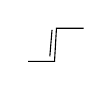
\begin{tikzpicture}[x=1em,y=1em]
\draw (0,0)--(.95,0)--(1.02,1.2)--(2,1.2);
\draw (.78,.18)--(.86,1.14);
\end{tikzpicture}}

Comme le \deleted{\unsure{sg}} premier de ces signes est forcément $\varepsilon'_1=\varepsilon_1$, cela signifie que \deleted{l'écriture} la suite de signes est la $=$ que celle des $\varepsilon_1,\varepsilon_2,\ldots,\unsure{\varepsilon_r,|\varepsilon_{r'}}$ (à la longueur près). Mais mieux, que l'expression $(\unsure{*})$ de $\tau'$ est son unique expression réduite, donc que $s=r'$ (longueur utile de $\tau'$), et que les $\lambda_i$ sont les longueurs $\ell'_i$ des intervalles critiques de $I_{\tau'}$.

\deleted{Cela signifie \deleted{\unsure{donc}} aussi que $F$ est \unsure{une composée|un composé} (par $*$) de morphismes \deleted{\unsure{d'intervalles de}} \inserted{des intervalles de} transition de $I_\tau$ \unsure{;} Si on désigne par}
